\section{Result}
\label{Result}
Systems and tools to minimize duplication of RFID cards have been successfully constructed using Multi-Factor Authentication method with username, password and OTP codes and can provide more security than using one authentication factor. Using multiple stages of authentication will minimize the occurrence of duplication and fraud. By utilizing some of these Authentication steps make the security system better than ever before. And the existing recordings are more organized.
The results of this study users will get OTP code in each account that has been registered in accordance with the card owned. The code will be sent to the user's account. Users can access the account by logging into the IP that has been provided. Code will be obtained every time the user tapping in the morning. And Code will be verified at home hours. The system will match the code that has been previously submitted based on the user card.

From the experimental results obtained:
\begin{enumerate}
    \item 
    if the card has not been registered then the card can not be read by system and will notification "Card is not Register".
    \item
    If the inserted OTP code does not match the code sent to the feeding user's account it will be rejected by the system and on the LCD it will display the notification of 'Invalid OTP Code'.
    \item
    If the OTP code and the card is in accordance then the data will be stored and the LCD will show the notification 'Thank you'
    \item
    The system can only be accessed using a predefined IP that is 192.168.1.102
    \item
    OTP code will be different every day and will be automatically generated when user tapping.
\end{enumerate}

Here are the results of the OTP code that was successfully sent to the user's account or card owner.
\begin{figure}[ht]
\begin{center}
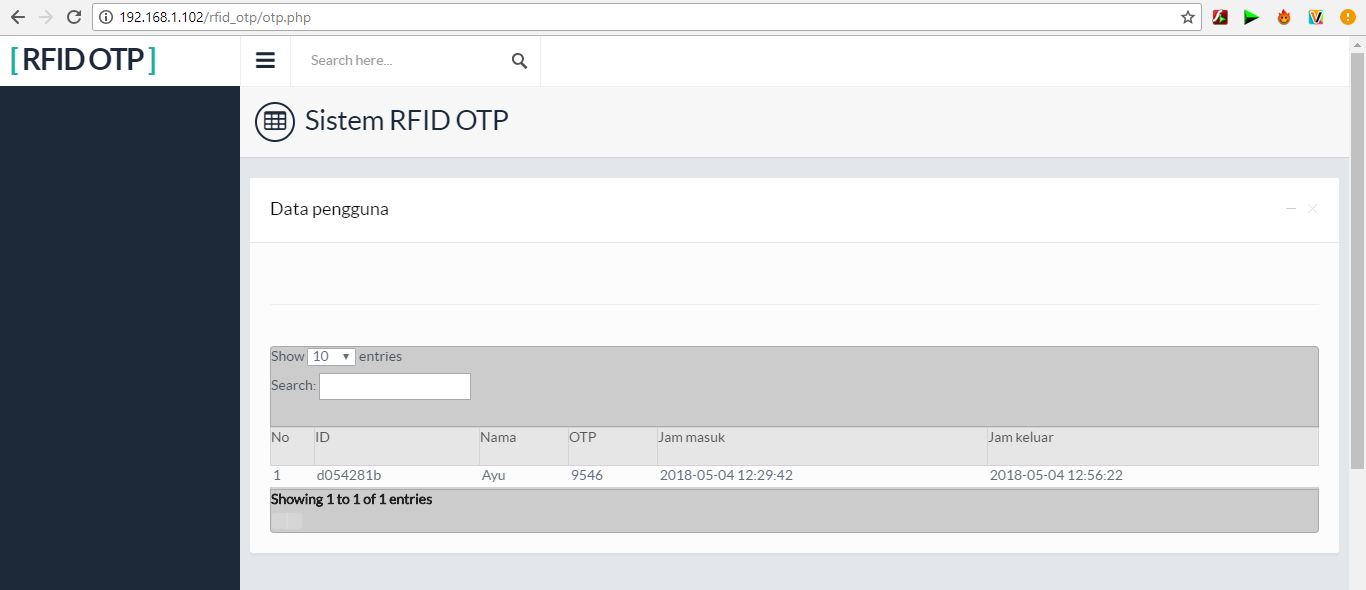
\includegraphics[width=12cm]{figures/OTP1.JPG}
\end{center}
\caption{User Account.
\label{eq:30}}
\end{figure}  

\begin{figure}[ht]
\begin{center}
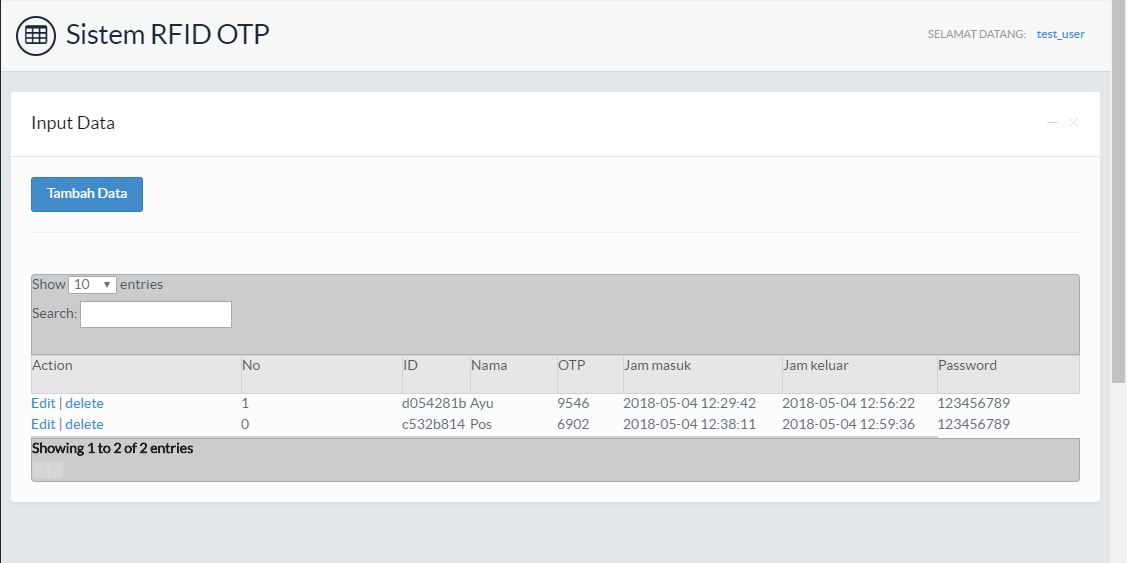
\includegraphics[width=12cm]{figures/AdminOTP.JPG}
\end{center}
\caption{Admin.
\label{eq:30}}
\end{figure}  


